\documentclass[a4,danish]{article}
\usepackage[a4paper, margin=3.5cm]{geometry}
% Standard library
\usepackage[utf8]{inputenc}
\usepackage[T1]{fontenc}
\usepackage{natbib, dsfont, enumitem,
  amssymb,soul,xcolor,amsmath,graphicx,subcaption,verbatim,pgfplots,tikz}
\usetikzlibrary{calc,patterns,angles,quotes,automata, positioning,arrows,shapes}

% Ref and bibliography style 
\bibliographystyle{abbrvnat}

% Handling new lines
\setlength{\parskip}{1em}
\setlength{\parindent}{0em}

% Handling space after sections
\usepackage{titlesec}
\titlespacing*{\section}{0em}{2em}{0em}
\titlespacing*{\subsection}{0em}{2em}{0em}
\titlespacing*{\subsubsection}{0em}{2em}{0em}

% No spacing after in start of list
\setlist[itemize]{topsep=0pt}
\setlist[enumerate]{topsep=0pt}

% Todo and notes
\usepackage[author=]{fixme}
\fxusetheme{color}
\definecolor{fxtarget}{rgb}{1,0.6,0}
\definecolor{fxnote}{rgb}{1,0.6,0}

\newcommand{\darkmode}[1]{ % Set dark mode or not
  \ifthenelse{ \equal{#1}{1}}{
    \usepackage{pagecolor}
    \definecolor{pagecol}{RGB}{0,43,54}
    \definecolor{textcol}{RGB}{131,148,150}
    % \definecolor{textcol}{RGB}{38,139,210}
    \pagecolor{pagecol}
    \color{textcol}
  }
}
% New operators and commands
\newcommand{\Z}{\mathbb{Z}}
\newcommand{\Q}{\mathbb{Q}}
\newcommand{\R}{\mathbb{R}}
\newcommand{\N}{\mathbb{N}}
\newcommand{\C}{\mathbb{C}}
\renewcommand{\S}{\mathbb{S}}
\newcommand{\blank}{\makebox[1ex]{\textbf{$\cdot$}}}
\newcommand\independent{\protect\mathpalette{\protect\independenT}{\perp}}
\def\independenT#1#2{\mathrel{\rlap{$#1#2$}\mkern2mu{#1#2}}}
\renewcommand{\phi}{\varphi}
\renewcommand{\epsilon}{\varepsilon}
\newcommand*\diff{\mathop{}\!\mathrm{d}}
\newcommand{\weakly}{\rightsquigarrow}
\newcommand\smallO{
  \mathchoice
    {{\scriptstyle\mathcal{O}}}% \displaystyle
    {{\scriptstyle\mathcal{O}}}% \textstyle
    {{\scriptscriptstyle\mathcal{O}}}% \scriptstyle
    {\scalebox{.6}{$\scriptscriptstyle\mathcal{O}$}}%\scriptscriptstyle
}
\newcommand{\midd}{\; \middle|\;}
\newcommand{\1}{\mathds{1}}
\usepackage{ifthen} %% Empirical process with default argument
% \newcommand{\G}[1][]{%
%    \ifthenelse{ \equal{#1}{} }
%       {\ensuremath{\mathbb{G}_n}}
%       {\ensuremath{\mathbb{G}_{#1}}}
% }
% New version:
\newcommand{\G}[2][n]{
{\ensuremath{\mathbb{G}_{#1}}{\left[#2\right]}}
}
\DeclareMathOperator*{\argmin}{\arg\!\min}

% New operators for consistent notation
\newcommand{\V}{\mathrm{Var}} % variance
\newcommand{\measure}[1]{\mathrm{{#1}}} % measure
% \newcommand{\measure}[1]{\textnormal{\textbf{{#1}}}} % measure
\newcommand{\m}[1]{\measure{#1}} % measure shortcut
\newcommand{\eqd}{\stackrel{d}{=}} % equality in distribution
\newcommand{\arrowP}{\xrightarrow{\; \m{P} \;}} % convergence in probability
\newcommand{\leb}{\lambda} % the Lebesgue measure
\newcommand{\T}{\top} % transpose

\usepackage{xargs}
% Make it easy to change counterfactual notation:
\newcommandx{\cf}[4][3={}, 4={}]{
  % \ifthenelse{ \equal{#4}{} }
  % {{#1^{#2}}(#3)}
  {\ifthenelse{ \equal{#3}{} }
    {{#1^{#2}}_{#4}}
    {{#1^{#2}}_{#4}(#3)}}
}

% Easily change notation:
\DeclareMathOperator{\TT}{\Psi} % target parameter
\newcommand{\lp}{\mathcal{L}_{\P}^2} % shortcut for lp2 space
\newcommand{\empmeas}{\hat{\mathbb{P}}_n} % empirical measure
\DeclareMathOperator{\E}{\mathbb{E}} % expectation
\renewcommand{\P}{\m{P}} % probability
\newcommand{\ic}{\mathrm{IF}} % influence curve
% Testing!:
% Def, theorems, etc. -- maybe review this
\usepackage{amsthm}

% Style separating env slightly from the rest
\newtheoremstyle{break}  
	{\topsep}{\topsep}
	{}{}
	{\bfseries}{}
	{\newline}{}
% Adjusted thm-environment with bullet at end
\newcommand{\newmarkedtheorem}[1]{%
  \newenvironment{#1}
    {\pushQED{\leavevmode\unskip\penalty9999 \hbox{}\nobreak\hfill
  \quad\hbox{\(\bullet\)}}
    \csname inner@#1\endcsname}
    {\popQED\csname endinner@#1\endcsname}%
  \newtheorem{inner@#1}%
}

\theoremstyle{plain} % plain italic style
\newtheorem{theorem}{Theorem}
\numberwithin{theorem}{section}
\newtheorem*{theorem*}{Theorem}
\newtheorem{conjecture}{Conjecture}
\newtheorem{lemma}[theorem]{Lemma}
\newtheorem{proposition}[theorem]{Proposition}
\newtheorem{corollary}[theorem]{Corollary}

\theoremstyle{definition} % non-italic
\newtheorem{definition}[theorem]{Definition}
% \newmarkedtheorem{definition}[theorem]{Definition}
\newtheorem{assumption}[theorem]{Assumption}
\newtheorem*{assumption*}{Assumption}
      
\theoremstyle{break}
\newmarkedtheorem{example}[theorem]{Example}
\newmarkedtheorem{note}[theorem]{Note}

\theoremstyle{remark}
\newmarkedtheorem{remark}[theorem]{Remark}
\makeatletter         
\renewcommand\maketitle{  
  {\raggedright
        \begin{flushright}
          {\color{white} 1} \\[-2cm] \@date % ... very hackish solution...
    \end{flushright}
    \begin{center}          
      {\LARGE  \@title}\\[2ex]
      \@author\\[6ex]
    \end{center}
}}
\makeatother
\fxsetup{status=final}
\usepackage[colorlinks=true]{hyperref} % Doesn't work for org, so included here

% For dark mode:
\darkmode{0}

\title{Influence functions and functional derivatives}
\author{Helene Rytgaard and Anders Munch}
\date{\today}

\begin{document}
\maketitle

\fxnote[inline, nomargin]{I think it is important to point out that this is background material.
  They are not supposed to understand everything fully and, particularly, they are not supposed to
  write like this in their reports (maybe only be able to grasp it intutively?). Moreover, I think
  for the last section we should focus on the ATE? As part of that particularly
  present the efficient influence function for the ATE.}

In this note we provide some motivation for studying influence functions and semiparametric
efficiency theory, and we briefly introduce the main theoretical concepts needed to study these
topics. For concreteness we relate the discussion to the specific problem of estimating the average
treatment effect (ATE), which we introduce in section~\ref{sec:introduction}. In
section~\ref{sec:motivation} we demonstrate how a naive (non-targeted) estimation procedure can
fail, and then give some heuristics that indicate a strategy for remedying this; in particular, we
will see that we would like to be able to talk about the \textit{derivative of a functional} defined
on a collection of probability measures. Hence in subsection~\ref{sec:funct-deriv} we first make
some general considerations about how to define a functional derivative, and then zoom in on the
statistical setting in subsections~\ref{sec:tang-spac-grad} and \ref{sec:prop-canon-grad}. These
subsections of section~\ref{sec:funct-deriv-can-grad} are slightly technical; this is because the
goal is to collect mathematically precise definitions and statements from the semiparametric
literature, which can be hard to find in compact form elsewhere. The main point to take away from
this section is that, given a statistical model $\mathcal{P}$ and a target parameter
$\theta = \TT(\P)$ defined through the functional $\TT \colon \mathcal{P} \rightarrow \R$, it is
possible to define the derivative of $\TT$. This derivative is referred to as the \textit{canonical
  gradient} and has two important properties (propositions~\ref{prop:eif-no} and \ref{prop:cr}),
which in turn imply that estimators based on the canonical gradient will asymptotically have
\textit{vanishing first order bias} and be \textit{efficient}. This is demonstrated in
section~\ref{sec:estim-based-canon} where we also present the canonical gradient for the ATE
problem. In section~\ref{sec:further-directions} we very briefly mention further directions and
related topics that are neglected in this note.

\fxnote[inline, nomargin]{[Notation]}


\section{The average treatment effect as a statistical problem}
\label{sec:introduction}

Many statistical problems are naturally formulated using one or more so-called \textit{nuisance
  parameters}. A nuisance parameter is a components we need to introduce in our the statistical
model, which is not of interest in itself, but is nevertheless needed to model the question of
interest. First of all let us note that by a \textit{statistical problem} we formally mean the tuple
$(\mathcal{P}, \TT)$, where $\mathcal{P}$ is a collection of probability measures and
$\TT \colon \mathcal{P} \rightarrow \R$ is a functional defined on this collection of probability
measures. The definition of $\mathcal{P}$ determines what kind of assumptions we make, while $\TT$
is determined by our scientific question of interest. 

We are particularly interested in statistical problems with infinite-dimensional nuisance parameter.
A good example of this the average treatment effect (ATE) which will be our running example
throughout.

\begin{example}[ATE]
  \label{example:aver-treatm-effect}
  Suppose we observed independent and identically distributed (iid) samples \(O_1,\ldots,O_n\),
  \(n\in\mathbb{N}\) of a random variable \(O \in\mathcal{O}\) distributed according to an unknown
  distribution function \(\P\) belonging to a statistical model \(\mathcal{P}\). Each observation
  consists of \(O= (X, A, Y)\) where \(X\in \R^d\) are covariates, \(A\in \lbrace 0,1\rbrace\) is a
  binary exposure and \(Y\in\lbrace 0, 1\rbrace\) is a binary outcome variable. The target parameter
  can be written as the functional \(\TT \colon \mathcal{P} \rightarrow \R\) on distributions
  \(\P\in\mathcal{P}\), for our purposes defined as
  \begin{align}
    \TT(\P) = \TT_1( \mu_X, f) = \int \big( f( 1, x) - f(0, x) \big) d\mu_X (x), 
    \label{eq:Psi:ate}
  \end{align}
  where \(f (a, x) = \E_{\P} [ Y \mid A=a, X=x]\) and \(\mu_X \) is the marginal distribution of
  \(X\), where we suppress the dependence on $\P$. Here we have used a subscript to differentiate
  between the functional $\TT$ considered as a map defined on $\mathcal{P}$ and the functional
  $\TT_1$ considered as a map defined on a product space containing $(\mu_X, f)$.
\end{example}

\fxnote*{ref}{The ATE can be interpreted causally under structural assumptions}. In this note, we do
not consider these important issues, but merely consider the estimation of the ATE as a statistical
problem as introduced above, i.e., a tuple $(\mathcal{P}, \TT)$ taking the concrete form given in
(\ref{eq:Psi:ate}). In this case, the nuisance parameters are the conditional expectation of the
outcome $Y$ given covariates $X=x$ and treatment $A=a$, which we denoted by $f$, and the marginal
distribution of $X$; we are not really interested in these functions, but we need them to be able to
express the ATE.

We note here that we could also have expressed or ``parametrized'' the target parameter differently:
Using iterated expectations it is straightforward to show both that $\TT(\P) = \TT_2(\mu, \pi)$ and
$\TT(\P) = \TT_3(\mu, f, \pi)$, where
\begin{align*}
  \TT_2(\mu, \pi) & := \int 
                    \left\{
                    \frac{a\,y}{\pi(x)} - \frac{(1-a)\,y}{1-\pi(x)} 
                    \right\}\diff \mu(y,a,x),\\
  \TT_3(\mu, f, \pi) &:=
                       \int 
                       \left\{
                       \frac{a\,(y-f(x,1))}{\pi(x)} + f(x,1) - \frac{(1-a)\,(y-f(x,0))}{1-\pi(x)} - f(x,0)
                       \right\}\diff \mu(y,a,x),
\end{align*}
with $\pi(x) := \P(A=1 \mid X=x)$ denoting the conditional probability of treatment given covariate
status. Hence, using $\TT_2$ the nuisance parameters would instead be the treatment mechanism $\pi$
and the full measure $\mu$, while using $\TT_3$ the nuisance parameters would be $f$, $\pi$, and
$\mu$. For later reference we define
\begin{equation}
  \label{eq:ate-pars}
  \begin{gathered}
    \phi_1(x; f) := f(1,x) - f(0,x), \quad
    \phi_2(y,a,x; \pi) := \frac{a\,y}{\pi(x)} - \frac{(1-a)\,y}{1-\pi(x)},\quad \text{and}  \\
    \phi_3(y,a,x; f, \pi) := \phi_2(y,a,x; \pi) + \phi_1(x; f) - \frac{a\,f(1,x)}{\pi(x)} +
    \frac{(1-a)\,f(0,x)}{1-\pi(x)},
  \end{gathered}
\end{equation}
% \begin{equation}
%   \label{eq:ate-pars}
%   \begin{split}
%     & \phi_1(x) :=   f(1,x) - f(0,x) \\
%     & \phi_2(y,a,x) :=   \frac{a\,y}{\pi(x)} - \frac{(1-a)\,y}{1-\pi(x)} \\
%     & \phi_3(y,a,x) := \phi_2(y,a,x) + \phi_1(x) - \frac{a\,f(1,x)}{\pi(x)} +
%     \frac{(1-a)\,f(0,x)}{1-\pi(x)},
%   \end{split}
% \end{equation}
such that we can write $\TT(\P) = \P[\phi_1(O, f)] = \P[\phi_2(O, \pi)] = \P[\phi_3(O, f, \pi)]$.

Statistical problems involving nuisance parameters lead to an obvious two-step estimation strategy:
\begin{enumerate}[label=(\arabic*), topsep=0pt]
\item Estimate the nuisance parameters.
\item Plug the estimates into the target parameter functional $\TT$.
\end{enumerate}
For instance, when estimating the ATE and using the parametrization in (\ref{eq:Psi:ate}), we would
(1)~estimate the conditional outcome $f(x,y) =\E[Y \mid A=a, X=x]$ and the marginal distribution
$\mu_X$ with estimators $\hat{f}_n$ and $\hat{\mu}_n$, and then (2)~plug these into $\TT_1$.
Estimation of $\mu_X$ is straightforward using the empirical measure $\empmeas$, which gives the
estimator
\begin{equation}
  \label{eq:naiv-est}
  \hat{\theta}_n = \TT_1(\empmeas, \hat{f}_n) 
  = \frac{1}{n} \sum_{i=1}^{n} 
  \left\{
    \hat{f}_n(1, X_i) - \hat{f}_n(0, X_i)
  \right\},
\end{equation}
where $\hat{f}_n$ is some estimated regression function, for instance obtained by linear regression.
Using instead the parametrization given by $\TT_2$ would demand estimation of $\pi$ in step (1),
giving the estimator $\TT_2(\empmeas, \hat{\pi}_n) $, while using $\TT_3$ would demand estimation of
both $f$ and $\pi$, giving the estimator $\TT_3(\empmeas, \hat{f}_n, \hat{\pi}_n) $.

Now, does it really matter which of these parametrizations we pick? And could we not just choose any
of them and then instead focus on picking a good nuisance estimator? Note that both estimation of
$f$ and $\pi$ are well-studied problems: The first is a regression problem while the second is a
classification problem, so we have a whole zoo of possible estimators, containing everything from
linear regression models to random forests, neural networks, etc. Should we not simply focus on
finding the best possible estimator of, say, $f$, and then just plug that into $\TT_1$? The example
in the following section \fxnote*{better formulation...}{demonstrates that some additional thought
  might be needed}.

\section{Motivation}
\label{sec:motivation}


%\begin{example}
%  \label{example:kernel-cdf}
To motivate our theoretical considerations on estimation of the ATE in this note, consider the
following simple toy example.

\begin{example}[Integrated kernel]
  \label{example:kernel-int}
  Given $n$ samples $X_i \in \R$ from some unknown distribution with cumulative distribution
  function $F$, we want to estimate $F(x) = \P(X \leq x)$. Let us say that we are willing to assume
  that $F$ has a continuous Lebesgue-density $f$. Then one estimation strategy would be to first use
  a kernel density estimator to estimate $f$, and then plug this into the integral operator
  \begin{equation*}
    f \longmapsto \int_{-\infty}^x f(z) \diff z,
  \end{equation*}
  to obtain an estimate of the cumulative distribution function $F(x)$ at the fixed point
  $x \in \R$. In this setting our nuisance parameter is $f$, and our target parameter is
  $\theta = \TT(f)$ with
  \begin{equation*}
    \TT \colon \mathcal{F} \rightarrow \R, \quad \TT(f) = \int_{-\infty}^x f(z) \diff z,
  \end{equation*}
  where $\mathcal{F}$ is some suitable function space, for instance the collection of continuous
  functions. This procedure results in the target and nuisance estimators given as
  \begin{equation}
    \hat{\theta}_n := \int_{-\infty}^x \hat{f}_n(z)  \diff z,
    \quad \text{and} \quad
    \hat{f}_n(z) = \empmeas[k_h(z, \blank)],
  \end{equation}
  for some kernel function $k_h$ with bandwidth $h_n$. It is well-known that the optimal choice of
  bandwidth $h_n$ is $h_n \propto n^{-1/5}$ \citep{wasserman2006all}, so this would also be the
  natural choice in our case; indeed, the upper panel of figure~\ref{fig:kernel-undersmoothed}
  demonstrates how this choice of bandwidth is superior to the choice $h_n \propto n^{-1/2}$, which
  instead results in a very rough or undersmoothed estimate.
  \begin{figure}[h]
    \centerline{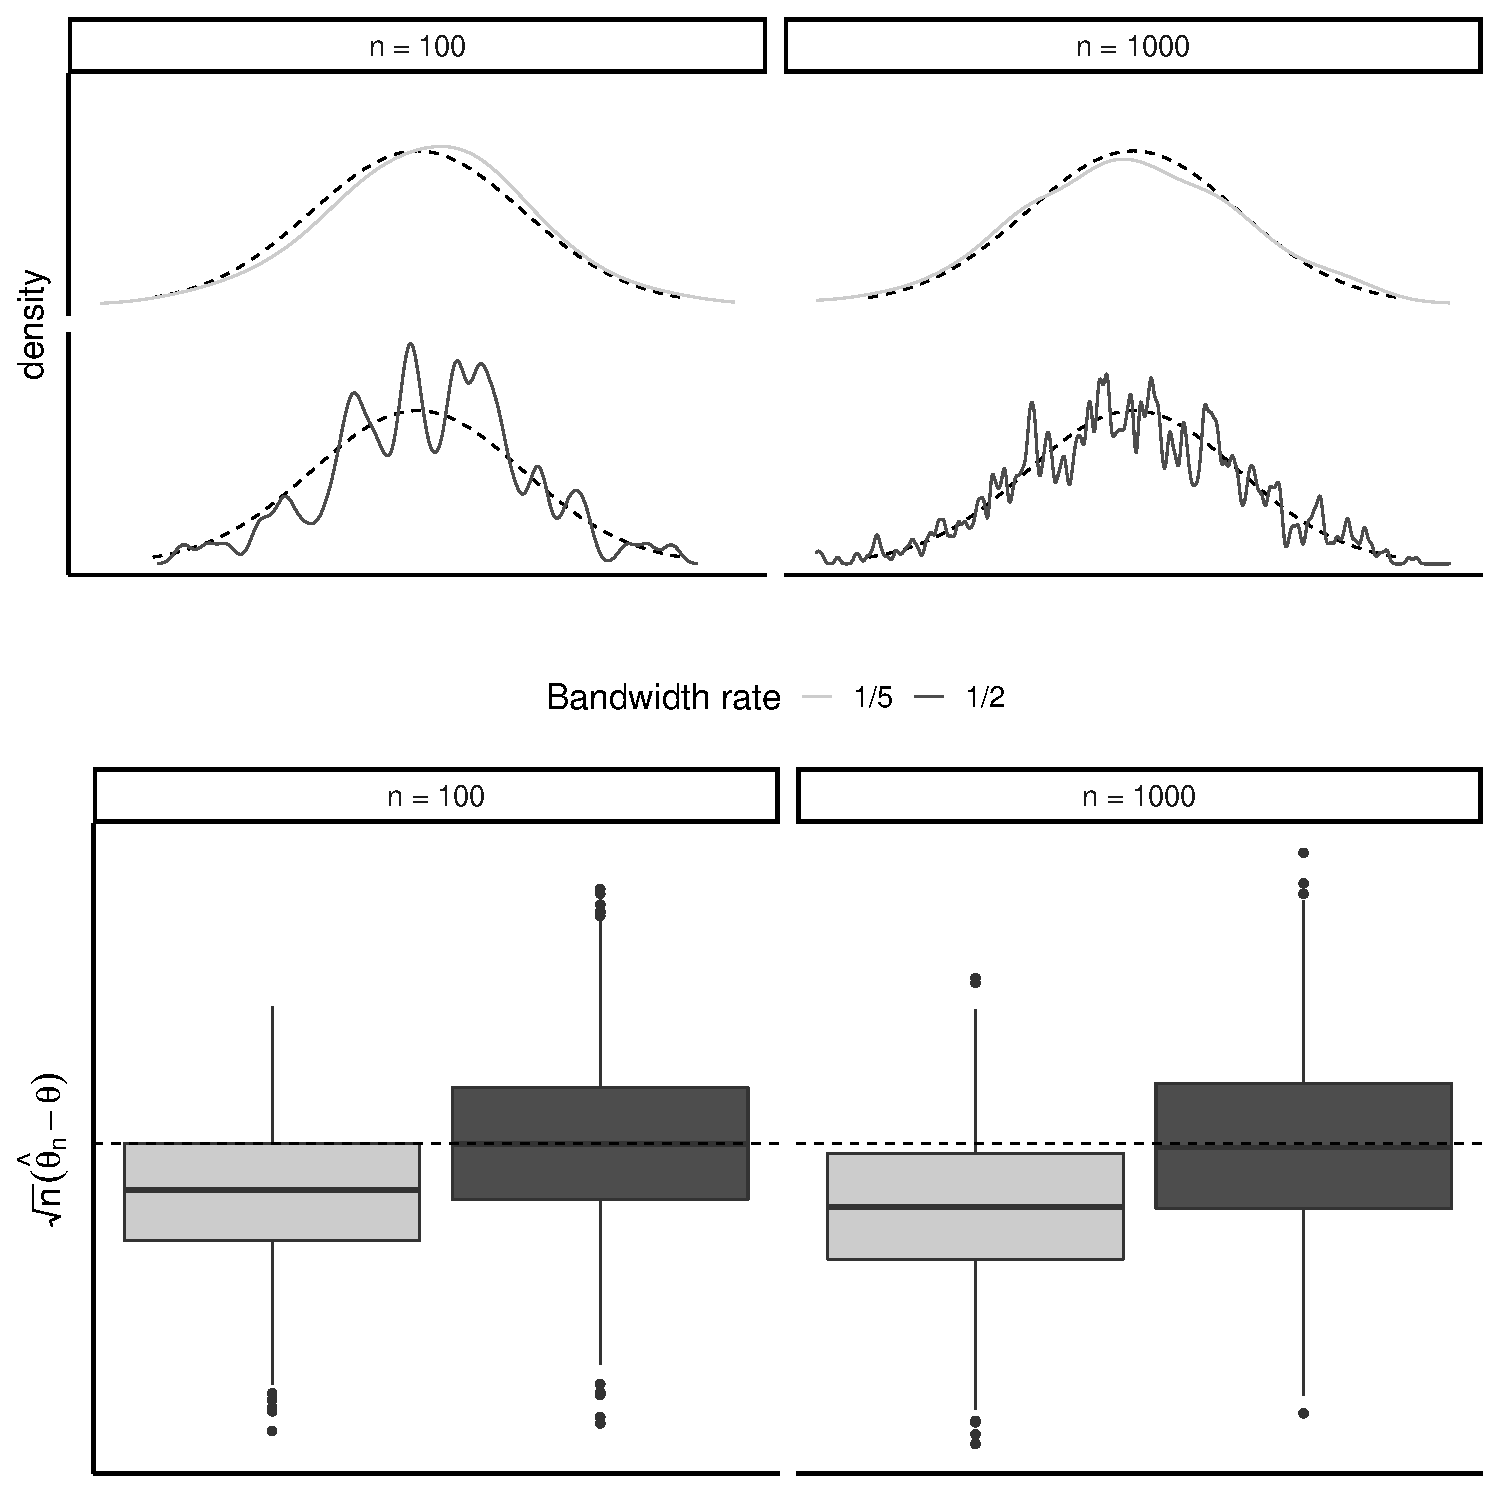
\includegraphics[width=.75\linewidth]{./figures/kernel-undersmooth-viz-presentation-3.pdf}}
    \caption{Simulation illustrating the problem for the plug-in approach. The top 2 rows give
      representative kernel density estimates for two different bandwidths scaling with $n$; the
      dashed line is the density of the distribution used to generate the data. The last row gives
      the distribution of the centralized and $\sqrt{n}$-scaled corresponding plug-in estimates
      based on 1000 Monte Carlo samples.}
    \label{fig:kernel-undersmoothed}
  \end{figure}
  Surprisingly, however, the lower panel shows that for estimation of the \textit{target parameter},
  plugging the undersmoothed estimate into $\TT$ is superior to using the default, optimal bandwidth
  estimator. \fxnote*{Add explicit bias variance decomposition?}{This example is in fact simply
    enough to allow an exact analytic calculation of the bias and variance of the target parameter,
    and hence it is fairly straightforward to mathematically prove the behavior suggested by
    figure~\ref{fig:kernel-undersmoothed}.}
\end{example}


Though the above example is somewhat silly because we already have an obvious estimator of the
parameter of interest in this situation, it clearly illustrates that the modus operandi outlined in
the two-step estimation procedure in the previous section can be problematic. With this example in
mind, we should maybe not be too confident about the first ATE estimator we considered
in~(\ref{eq:naiv-est}). In fact, with a bit more work it can be showed that the same phenomenon as
illustrated in figure~\ref{fig:kernel-undersmoothed} appears if we use a kernel-based regression
estimator in~(\ref{eq:naiv-est}). 

The issue from the toy example can be understood more generally by considering a target parameter
$\TT$ that can be parametrized as $\TT(\P) = \TT_0(\P, \nu) = \P[\phi(O, \nu)]$ for some function
$\phi(\blank, \nu)$ defined on the sample space $\mathcal{O}$ that depend on the nuisance parameter
$\nu$. (Many target parameters can be written on this form; in particular, as shown above, the ATE
can be written on this form in at least three different ways.) Plugging the nuisance estimators
$\empmeas$ and $\hat{\nu}_n$ into this expression gives the estimator
$\hat{\theta}_n = \TT_0(\empmeas, \hat{\nu}_n)$. To analyze the (asymptotic) behavior of this
estimator we would typically consider the expression
\begin{equation*}
  \sqrt{n}
  \left(
    \hat{\theta}_n - \theta
  \right)
  =  \sqrt{n}
  \left(
    \TT_0(\empmeas,\hat{\nu}_n) - \TT_0(\P,\nu)
  \right) =
  \sqrt{n}
  \left(
    \empmeas[\phi(O, \hat{\nu}_n)] -
    \P[\phi(O, \nu)]
  \right),
\end{equation*}
which can be further expanded as
\begin{align*}
  \sqrt{n}
  \left(
  \hat{\theta}_n - \theta
  \right) & =
            \G{\phi( O, \hat{\nu}_n)}
            + \sqrt{n}
            \left\{
            \TT_0(\P,\hat{\nu}_n) - \TT_0(\P,\nu)
            \right\},
  % \\
  %         & = \G{\phi( \blank, \hat{\nu}_n)}
  %           + \sqrt{n}
  %           \left\{
  %           \mathrm{D}_{\nu}{\TT}(\hat{\nu}_n - \nu)
  %           + \mathcal{O}_{\P}(\Vert \hat{\nu}_n - \nu \Vert^2)
  %           \right\},
\end{align*}
where $\mathbb{G}_n$ denotes the empirical process defined as
$\mathbb{G}_n := \sqrt{n}(\empmeas - \P)$. Let us now consider some heuristic arguments: If we could
somehow make sense of a Taylor expansion of the function $\nu \mapsto \TT_0(\P, \nu)$ we could
further expand the above as
\begin{equation}
  \label{eq:target-decom}
  \sqrt{n}
  \left(
    \hat{\theta}_n - \theta
  \right)
  = \G{\phi( O, \hat{\nu}_n)}
  + \mathrm{D_{\nu}{\TT_0}}{ \left[
      \sqrt{n}(\hat{\nu}_n - \nu)
    \right]}
  + 
  \mathcal{O}_{\P}(\sqrt{n}\Vert \hat{\nu}_n - \nu \Vert_{\mathcal{V}}^2),
\end{equation}
where $\Vert \blank \Vert_{\mathcal{V}}$ is some norm defined on the space where the nuisance
parameter $\nu$ takes it values; this would typically be a function space, so the norm could, for
instance, be the $\mathcal{L}^2$-norm or the supremum-norm. The asymptotic analysis of each of the
three components in (\ref{eq:target-decom}) requires some fairly advanced mathematical tools, and in
this note we only focus on the second part. For the other two components we simply note that in many
cases empirical process theory or sample splitting can be used to show that
$\G{\phi(O, \hat{\nu}_n)} = \G{\phi(O, \nu)} + \smallO_{\P}(\sqrt{n})$, and that
$\Vert \hat{\nu}_n - \nu \Vert_{\mathcal{V}} = \smallO_{\P}(n^{-1/4})$ \fxnote*{is this
  correct?}{has been established for several machine learning estimators} under the right conditions
(see section~\ref{sec:further-directions} for a few additional comments on this). Assuming this two
equations to hold, (\ref{eq:target-decom}) simplifies to
\begin{equation*}
  \sqrt{n}
  \left(
    \hat{\theta}_n - \theta
  \right)
  = \G{\phi( O, \nu)}
  + \mathrm{D_{\nu}{\TT_0}}{ \left[
      \sqrt{n}(\hat{\nu}_n - \nu)
    \right]}
  + 
  \smallO_{\P}(1).  
\end{equation*}
The first component is now straightforward to analyze using the central limit theorem, as it is a
sum of iid.\ zero-mean variables. This term contributes the main part of the variance of the
asymptotic behavior of $\hat{\theta}_n$. The second component can contribute with additional
variance, if the $\hat{\nu}_n$ converges at $n^{-1/2}$-rate; however, if $\hat{\nu}_n$ converges at
a slower rate, the main issue with the second component becomes bias. Indeed, as the default kernel
estimator converges \fxnote*{check}{at rate $n^{-2/5}$}, this component is exactly what ruined the
target estimator in example~\ref{example:kernel-int}. If we want to use flexible, non-parametric
nuisance estimators we can in general not hope to be able to have these converge at the parametric
$n^{-1/2}$-rate (for instance, the $n^{-2/5}$-rate is the best possible for estimation of twice
times continuously differentiable densities \citep[chp.~24]{van2000asymptotic}). Hence we cannot
hope to achieve $n^{-1/2}$-rate inference about $\theta$ by optimizing the nuisance parameter, and
thus we instead turn to the derivative $\mathrm{D_{\nu}{\TT_0}}$. In particular, if we can design
$\TT_0$ in such a way that $\mathrm{D_{\nu}{\TT_0}} = 0$, we would get rid of this problematic bias
term altogether.

This goal is our motivation for studying functional derivatives in the next section. As mentioned,
we will see that this study will also allow us to analyze how efficiently a given statistical
problem can be estimated.

\section{Functional derivatives and the canonical gradient}
\label{sec:funct-deriv-can-grad}

For infinite-dimensional spaces, unlike for $\R^d$, there are several sensible and non-equivalent
ways of defining a derivative. In addition, again unlike for $\R^d$, for such spaces there are
typically several, non-equivalent norms, which in turn determine which kind of functionals and
operators are differentiable according to what definition. We do not consider these issues in much
detail but only consider two types of derivatives, namely Gâteaux and Hadamard. We then consider
some slight generalizations of the latter, and then, in subsection~\ref{sec:tang-spac-grad},
describe in greater detail how Hadamard derivatives for a statistical problem can be represented;
this allow us to derive some useful properties in subsection~\ref{sec:prop-canon-grad}.

\subsection{Functional derivatives}
\label{sec:funct-deriv}

The most straightforward form of functional differentiabiliy is the generalization of the
\textit{directional derivative} of multivariate calculus. This is known as Gâteaux differentiability
and defined as follows.

\begin{definition}[Gâteaux derivative]
  Let $\mathcal{M}$ and $\mathcal{Y}$ be a normed real vector spaces,
  $\TT \colon \mathcal{M} \rightarrow \mathcal{Y}$ a map, and $x \in \mathcal{M}$ a point in the
  domain. If there exists a linear, continuous operator
  $\dot{\TT}_x \colon \mathcal{M} \rightarrow \mathcal{Y} $ such that for all $h \in \mathcal{M}$
  \begin{equation*}
    \left\Vert
      \TT(x + \epsilon h) - \TT(x) - \dot{\TT}_x(\epsilon h)
    \right\Vert_{\mathcal{Y}} = \smallO(\epsilon),
    \quad \text{when} \quad \epsilon \longrightarrow 0 \in \R,
  \end{equation*}
  we say that $\TT$ is Gâteaux differentiable at $x$. We call the operator $\dot{\TT}_x$ the
  Gâteaux derivative of $\TT$ at $x$.
\end{definition}

If the map $\TT$ is Gâteaux differentiable at $x$ then it follows from the definition that
\begin{equation}
  \label{eq:1}
    \left\Vert
      \frac{\TT(x + \epsilon h) - \TT(x)}{\epsilon} - \dot{\TT}_x(h)
    \right\Vert_{\mathcal{Y}} \longrightarrow 0,
    \quad \text{when} \quad \epsilon \longrightarrow 0.
\end{equation}
In particular, when $\mathcal{Y} = \R$ the Gâteaux derivative at $x$ in the direction $h$ can be
derived as the ordinary derivative of the real-valued function
$\epsilon \mapsto \TT(x + \epsilon h)$ evaluated at 0, i.e.,
\begin{equation}
  \label{eq:gateaux-prop}
  \dot{\TT}_x(h) = \partial_0{\TT(x + \epsilon h)}
  := \frac{\partial}{\partial \epsilon} \bigg \vert_{\epsilon=0}{\TT(x + \epsilon h)}.
\end{equation}
To simplify notation in the following we will use the notation \fxnote*{hely would like to change
  this notation}{$\partial_0{f(\epsilon)}$} for maps $f$ with a real domain as just defined in
(\ref{eq:gateaux-prop}). Gâteaux differentiability is used by \cite{chernozhukov2018double} to
define \textit{Neyman orthogonality}: A function
$\phi \colon \mathcal{O} \times \mathcal{V}\rightarrow \R$, defined on the sample space
$\mathcal{O}$ and depending on a nuisance parameter $\nu \in \mathcal{V}$, fulfills \fxnote*{proper
  definition or is this fine?}{the Neyman orthogonality condition (wrt.\ $\mathcal{V}$)} if the map
\begin{equation*}
  F \colon \mathcal{V} \longrightarrow \R, \quad \nu \longmapsto F(\nu) :=  \TT_0(\P, \nu) =\P[\phi(O, \nu)]
\end{equation*}
is Gâteaux differentiable at $\nu$ with vanishing derivative, i.e., $\dot{F}_{\nu}(h) = 0$ for all
$h \in \mathcal{V}$. We encountered the map above in section~\ref{sec:motivation}, and the point of
Neyman orthogonality is exactly to ensure that the second component of the decomposition in
(\ref{eq:target-decom}) vanishes. Given a function $\phi$ it is straightforward to use
(\ref{eq:gateaux-prop}) to verify that a given function fulfills the condition. Indeed, one can
examine $\phi_1$, $\phi_2$, and $\phi_3$ defined in (\ref{eq:ate-pars}) and see that $\phi_3$
fulfills the Neyman orthogonality condition while $\phi_1$ and $\phi_2$ do not.

This shows that Gâteaux is already a useful concept. Still, it is a rather weak form of
differentiability; \fxnote*{better fomrlation}{for instance, as it is equivalent to the directional
  derivative for ordinary multivariate functions, Gâteaux differentiability is not enough to
  guarantee (ordinary) differentiability of such functions}. To get a richer theory, a stronger
notion of differentiability is needed. For our setting, a particular useful concept is
\textit{Hadamard} differentiability.

\begin{definition}[Hadamard derivative]
  \label{def:hadamard-diff}
  Let $\mathcal{M}$ and $\mathcal{Y}$ be a normed real vector spaces,
  $\TT \colon \mathcal{M} \rightarrow \mathcal{Y}$ a map, and $x \in \mathcal{M}$ a point in the
  domain. If there exists a linear, continuous operator
  $\dot{\TT}_x \colon \mathcal{M} \rightarrow \mathcal{Y} $ such that
  \begin{equation*}
    \left\Vert
      \frac{\TT(x + \epsilon_n h_n) - \TT(x)}{\epsilon_n} - \dot{\TT}_x(h)
    \right\Vert_{\mathcal{Y}} \longrightarrow 0,
  \end{equation*}
  for any $\epsilon_n \rightarrow 0$ and $\{h_n\}_{n \in \N} \subset \mathcal{M}$ with
  $h_n \rightarrow h \in \mathcal{M}$, we say that $\TT$ is Hadamard differentiable at $x$ and call
  the operator $\dot{\TT}_x$ the Hadamard derivative of $\TT$ at $x$.
\end{definition}

Comparing this definition with (\ref{eq:1}) we see that the only
difference is that the linear approximation provided by $\dot{\TT}_x$
should hold along any \textit{converging sequence} $h_n$ and not
merely in a fixed direction $h$. For this reason Hadamard
differentiability is also known a \textit{path-wise}
differentiability. A still stronger condition is to demand that the
approximation should hold for any \textit{bounded sequence} $h_n$;
this gives the concept of \textit{Fréchet} differentiability, which we 
will not use in this text. One can show that \textit{if} a map is
Hadamard (or Fréchet) differentiable, then the Hadamard (or Fréchet)
derivative is equal to the Gâteaux derivative. Hence, to find the
Hadamard derivative of a given functional $\TT$, the common strategy
is to first use high school math tools to calculate
(\ref{eq:gateaux-prop}) and then verify that the obtained candidate
fulfills the requirements of definition~\ref{def:hadamard-diff}.

So far we have assumed the domain to be a \textit{linear} space. When working with probability
measures, this is often not the case, and hence we need one final definition, which allows the
operator $\TT$ and its derivative $\dot{\TT}$ to be defined only on subsets of the normed vector
space $\mathcal{M}$. We should think of the following as mirroring differentiation of a multivariate
function defined on a manifold embedded in a higher dimensional Euclidean space \fxnote*{Make a
  picture}{(for instance, a surface embedded in $\R^3$)}.

\begin{definition}[Tangential Hadamard derivative]
  Let $\mathcal{P}$ and $\dot{\mathcal{P}}_x$ be subsets of the normed real vector space
  $\mathcal{M}$, with $x \in \mathcal{P} \subset \mathcal{M}$. For a map
  $\TT \colon \mathcal{P} \rightarrow \mathcal{Y}$, we say that $\TT$ is \textit{Hadamard
    differentiable (at $x$) tangential to $\dot{\mathcal{P}}_x$} if there exists a continuous,
  linear operator $\dot{\TT}_x \colon \dot{\mathcal{P}}_x \rightarrow \mathcal{Y}$ such that
  \begin{equation*}
    \left\Vert
      \frac{\TT(x + \epsilon_n h_n) - \TT(x)}{\epsilon_n} - \dot{\TT}_x(h)
    \right\Vert_{\mathcal{Y}} \longrightarrow 0, 
  \end{equation*}
  for any $\{h_n\} \subset \mathcal{M}$ and $\{\epsilon_n\} \subset \R$ with
  $h_n \rightarrow h \in \dot{\mathcal{P}}_x$, $\epsilon_n\rightarrow 0$, and
  $x + \epsilon_n h_n \in \mathcal{P}$.
\end{definition}

The only change from the previous definition is that the ``path'' $x + \epsilon_n h_n$ is restricted
to lie in the subset $\mathcal{P}$, and that the ``direction'' is $h$ is restricted to lie in
$\dot{\mathcal{P}}_x$.

\subsection{Tangent spaces and gradients for statistical problems}
\label{sec:tang-spac-grad}

Using the tools introduces so far, we can now define the so-called \textit{tangent space for the
  model $\mathcal{P}$} and then formally define the derivative of the map
$\TT\colon\mathcal{P} \rightarrow \R$ from the statistical problem $(\mathcal{P}, \TT)$. We refer to
this derivative as the \textit{canonical gradient}, or later in section~\ref{sec:estim-based-canon}
the \textit{efficient influence function}. The canonical gradient is a central component in our
analysis of the statistical problem as it represents the optimal asymptotic variance
(proposition~\ref{prop:cr}); in addition it allows us to construct estimators with vanishing first
order bias (proposition~\ref{prop:eif-no} and section~\ref{sec:estim-based-canon}).

As shown in the previous subsection, to be able to talk about differentiability of the statistical
problem $(\mathcal{P}, \TT)$, we need to embed the model $\mathcal{P}$ into a suitable normed vector
space. To do so we now assume for simplicity that the family $\mathcal{P}$ is dominated by a single
$\sigma$-finite measure $\mu$ (for our running example of the ATE this measure would be a product of
Lebesgue and counting measures), and then think of $\mathcal{P}$ as lying inside the Banach space
$\mathcal{M}_{\mu}$ of finite signed measures dominated by $\mu$ equipped with the variational norm
\begin{equation*}
  \Vert M \Vert_{\mathcal{M}_{\mu}} = \int |m |\diff \mu, \quad \text{ for } \quad M = m \cdot \mu.
\end{equation*}

\begin{definition}[Tangent space for $\mathcal{P}$]
  Let $\mathcal{P} \subset \mathcal{M}_{\mu}$ be a collection of probability measures and let
  $\P \in \mathcal{P}$. For any one-dimensional path
  $\epsilon \mapsto \P_{\epsilon} \in \mathcal{P}$ with $\P_0 =\P$, which is Hadamard\footnote{When
    the domain is $\R$, all the previously considered types of differentiability are equivalent, so
    any type could be used here.} differentiable at 0, let $\partial_0{\P_{\epsilon}}$ be the
  derivative, and let $\{\partial_0{\P_{\epsilon}}\}$ be the collection of derivatives of all such paths. We call
  the \fxnote*{should there be added some note about this -- always sensible thing, or need to
    assume something?}{closed linear span} of this collection the \textit{tangent space of
    $\mathcal{P}$ at $\P$} and denote it by $\dot{\mathcal{P}}_{\P}$. Formally,
  \begin{equation*}
    \dot{\mathcal{P}}_{\P}
    := \overline{\mathrm{span}}
    % {\dot{\mathcal{P}}_{\P}^0} , \quad 
    % \dot{\mathcal{P}}_{\P}^0    :=
    % \left\{ \frac{\diff}{\diff \epsilon } \Big\vert_{\epsilon=0} \P_{\epsilon}
    \left\{ \partial_0{\P_{\epsilon}}
      \midd \epsilon \mapsto \P_{\epsilon} \text{ is Hadamard differentiable and } \P_0 = \P  \right\}.
  \end{equation*}
\end{definition}

The definition of a tangent space for a collection of probability measures simple mimics the
definition of a tangent space for a surface embedded in $\R^3$: We move along differentiable paths
through a given point on the surface, and the tangent space is then the span of the derivatives of
all such paths. With a differentiable structure on the collection $\mathcal{P}$ we can talk about a
\textit{gradient} of a functional defined on this set.

\begin{definition}[Canonical gradient]
  \label{def:tangt-space-prob}
  Let $(\mathcal{P}, \TT)$ be a statistical problem, with $\mathcal{P} \subset \mathcal{M}_{\mu}$,
  and $\dot{\mathcal{P}}_{\P}$ the tangent space of $\mathcal{P}$ at $\P \in \mathcal{P}$. If
  $\TT \colon \mathcal{P} \rightarrow \R$ is Hadamard differentiable at $\P$ tangential to
  $\dot{\mathcal{P}}_{\P}$, we refer to the Hadamard derivative $\dot{\TT}_{\P}$ as the
  \textit{canonical gradient of the statistical problem}.
\end{definition}

The definitions of the tangent space $\dot{\mathcal{P}}_{\P}$ and the gradient $\dot{\TT}_{\P}$
above capture the intuitive meaning of these concepts as generalizations of well-known concepts from
multivariate calculus: The statistical model $\mathcal{P}$ is viewed as a subset of the unit sphere
in $\mathcal{M}_{\mu}$ and the canonical gradient $\dot{\TT}_{\P}$ is simply the
infinite-dimensional version of the gradient of a map defined on a surface in Euclidean space. We
shall see in a moment why this object $\dot{\TT}_{\P}$ is of interest for the statistician, but
firstly we consider a different representation of $\mathcal{P}$ which allows us to represent
$\dot{\mathcal{P}}_{\P}$ as a subset of $\lp$; this is particularly useful as we then
have the rich Hilbert space structure of $\lp$ at our disposal.

For a fixed element $\P \in \mathcal{P}$ with $\mu$-density $p$, consider a one-dimensional
parametric submodel of $\mu$-densities $p_{\epsilon}$ with $p_0=p$ and
$p_{\epsilon} \cdot \mu \in \mathcal{P}$ for all $\epsilon$ in some small interval. We restrict
attention to such submodels for which the score function
$\dot{\ell}_0 := \partial_0{\log(p_{\epsilon})}$ exists as an element in $\lp$; here we use the
terminology from ordinary maximum likelihood inference where the derivative of the likelihood for a
parametric model $p_{\epsilon}$ is referred to as the score function. We denote the closed linear
span of all such score functions by $\Gamma_{\P}$, i.e.,
$\Gamma_{\P} := \overline{\mathrm{span}}\{\dot{\ell}_0\} \subset \lp$, where $\{\dot{\ell}_0\}$ is
read as the collection of all possible score functions. \fxnote*{I would like to make this
  precise.}{It is argued by \cite{bickel1993efficient} that, for all relevant purposes,}
$\Gamma_{\P}$ is equivalent to the tangent space $\dot{\mathcal{P}}_{\P}$ from
definition~\ref{def:tangt-space-prob}, and hence $\Gamma_{\P}$ is also referred to as the tangent
space. It can be shown that all elements of $\Gamma_{\P}$ have mean zero (under $\P$), i.e.,
\begin{equation*}
  \Gamma_{\P} \subset \mathbb{H}_0 := 
  \left\{
    h \in \lp \mid \P[h] = 0
  \right\}, 
\end{equation*}
and that if we make no assumptions about the model $\mathcal{P}$ then $\Gamma_{\P} = \mathbb{H}_0$
\fxnote*{more precise reference}{\citep{bickel1993efficient}}.

Due to the well-known structure of $\lp$, is often easier to analyze the tangent space as the
subspace $\Gamma_{\P} \subset \lp$; for instance, one useful result is the following proposition,
which provides an alternative \fxnote*{as stated now, this is not exactly what the proposition
  says.}{characterization} of the canonical gradient.

% \begin{proof}
%   \fxnote*{todo/finish. Pretty sure this results is correct...}{Something like this:} We can also
%   represent $\mathcal{P}$ as a subset of $\mathcal{L}_{\mu}^2$ through the map
%   $\P \mapsto \sqrt{p}$, and the topology on $\mathcal{P}$ induced in this way is \fxnote*{check --
%     also the generalized versions on the whole space?}{the same as that induced} by
%   $\Vert \blank \Vert_{\mathcal{M}_{\mu}}$ \citep{bickel1993efficient}. This implies that
%   convergence of $(\P_{\epsilon h} - \P_{0})\epsilon^{-1}$ in $\mathcal{M}_{\mu}$ is equivalent to
%   convergence of convergence of $(\sqrt{p_{\epsilon h}} - \sqrt{p_{0}})\epsilon^{-1}$ in
%   $\mathcal{L}_{\mu}^2$. \fxnote*{finish}{Then Gâteaux + map with $/p_0$...}
% \end{proof}

\begin{proposition}
  \label{prop:repr-can-gradient}
  Let $(\mathcal{P}, \TT)$ be a statistical problem with canonical gradient
  $\dot{\mathcal{\TT}}_{\P}$ at $\P \in \mathcal{P}$. There exists a unique element
  $\phi_{\P} \in \Gamma_{\P}$ such that
  \begin{equation}
    \label{eq:2}
    \partial_0{\TT(\P_{\epsilon})}
    = \mathrm{\dot{\TT}_{\P}}
    {\left(
        \partial_{0}{\P_{\epsilon}} 
      \right)}
    = \langle \phi_{\P}, \dot{\ell}_0 \rangle_{\P}
    % =  \int \phi \dot{\ell}_0  \diff \P,
  \end{equation}
  holds for any differentiable submodel $\P_{\epsilon}$ with score function $\dot{\ell}_0$.
\end{proposition}

\begin{proof}[Sketch of proof]
  The first equality follows from the chain rule for Hadamard derivatives
  \citep[chp.~20]{van2000asymptotic}, while the second follows from the arguments given above: If
  the tangent space can be represented as $\Gamma_{\P}$, the linear map $\dot{\TT}_{\P}$ on
  $\dot{\mathcal{P}}_{\P}$ \fxnote*{make this proof precise}{can also be thought} of as a linear map
  on $\Gamma_{\P}$. As $\Gamma_{\P}$ is a closed subspace of a Hilbert space it is itself a Hilbert
  space, and hence Riesz representation theorem (for Hilbert spaces) gives the existence of a unique
  element $\phi_{\P} \in \Gamma_{\P}$ such that
  $\Phi_{\P}(\dot{\ell}_0) = \langle\phi_{\P}, \dot{\ell}_0\rangle$ for all elements
  $\dot{\ell}_0 \in \Gamma_{\P}$.
\end{proof}

As with the identification $\dot{\mathcal{P}}_{\P}= \Gamma_{\P}$ we also \fxnote*{}{identify} the
function $\phi_{\P}$ with the canonical gradient $\dot{\TT}_{\P}$. By the chain rule of ordinary
multivariate calculus we have for a differentiable function $f\colon\R^d \rightarrow \R$ and any
smooth curve $s\colon\R\rightarrow \R^d$ with $s(0) = x_0 \in \R^d$ that
\begin{equation*}
  \partial_0(f\circ s) = \nabla f(s(0)) \cdot (\partial_0{s} )^{\T}
  =
  \left\langle
    \nabla f(x_0) ,  \partial_t{s} 
  \right\rangle,
\end{equation*}
and as $\R^d$ can be spanned by smooth 1-dimensional curves, this property characterizes the
gradient locally. Proposition~\ref{prop:repr-can-gradient} above states that this characterization
extends to the Hilbert space setting with Hadamard differentiability, and in fact this
characterization \fxnote*{I think this is correct}{can be used to define} Hadamard differentiability
of the map $\TT$ tangential to $\Gamma_{\P}$ \citep[A.5]{bickel1993efficient}.

\begin{remark}
  \label{remark:gradients}
  Note that it is part of the defining property of the unique function $\phi_{\P}$ that it lies in
  the tangent space $\Gamma_{\P}$. If $\Gamma_{\P}$ is a proper subset of $\mathbb{H}_0$ there can
  be several functions $\tilde{\phi} \in \mathbb{H}_0$ fulfilling condition (\ref{eq:2}); we refer
  to such functions as \textit{gradients}. It follows from standard Hilbert space theory that the
  unique canonical gradient $\phi_{\P}$ can be derived from any gradient $\tilde{\phi}$ as the
  projection onto $\Gamma_{\P}$, i.e., $ \phi_{\P} = \Pi(\tilde{\phi} \mid \Gamma_{\P})$. This
  geometric picture of the tangent space and the canonical gradient can be very useful.
\end{remark}


\subsection{Properties of the canonical gradient}
\label{sec:prop-canon-grad}

In this subsection we derive two important properties of the canonical gradient. The first result
states that the canonical gradient fulfills the Neyman orthogonality condition, which is the same as
saying that the mean of the canonical gradient is insensitive to small (first order) perturbations
of the nuisance parameters. The second results states that the canonical gradient in addition
provides us with a theoretical bound on how efficient the target parameter can be estimated.

\begin{proposition}
  \label{prop:eif-no}
  Let $(\mathcal{P}, \TT)$ be a statistical problem with $\mathcal{P}$ dominated by $\mu$ and such
  that $\TT(\P) = \P[\phi(Z, \nu(\P))]$ for some function
  $\phi\colon \mathcal{Z} \times \mathcal{V} \rightarrow \R$. If
  $\phi(\blank, \nu(\P)) - \P[\phi(O, \nu(\P))]$ is the canonical gradient of $(\mathcal{P}, \TT)$
  at $\P$ then, \fxnote*{can these be made precise?}{under regularity conditions}, $\phi$ fulfills
  the Neyman orthogonality condition \fxnote*{ok? Or should it actually be
    $\dot{\nu}_{\P}(\dot{\mathcal{P}}_{\P})$?}{(wrt.\ $\nu(\mathcal{P})$)}.
\end{proposition}

\begin{proof}[Sketch of proof]
  Under suitable regularity conditions, it holds for any \fxnote*{}{differentiable} path
  $\{\P_{\epsilon}\}_{\epsilon} \subset \mathcal{P}$ with $\P_0=\P$ that
  \begin{align}
    \label{eq:3}
    \begin{split}
      \partial_0{ \TT(\P_{\epsilon})}% = \partial_0 \P_{\epsilon}[\phi(Z, \nu(\P_{\epsilon}))]
      & =\partial_0{ \int p_{\epsilon}(z) \phi(z, \nu(\P_{\epsilon})) \diff \mu(z)} \\
      & = \int p(z) \{\partial_0{ \phi(z, \nu(\P_{\epsilon}))}\} +  \{\partial_0{p_{\epsilon}(z)}\} \phi(z, \nu(\P)) \diff \mu(z) \\
      & = \partial_0{\P[ \phi(\blank, \nu(\P_{\epsilon}))]} +
      \langle \dot{\ell}_0, \phi(\blank, \nu(\P))\rangle_{\P},
    \end{split}
  \end{align}
  where $\dot{\ell}_0$ is the score function of the parametric submodel $\P_{\epsilon}$ and we used
  the relation $\partial_0{\log p_{\epsilon}} = (\partial_0{p_{\epsilon}})p_0^{-1}$. As
  $\phi(\blank, \nu(\P))$ is the canonical gradient at $\P$,
  proposition~\ref{prop:repr-can-gradient} and (\ref{eq:3}) imply that \fxnote*{enought? Finish the
    proof.}{$\partial_0{\P[ \phi(\blank, \nu(\P_{\epsilon}))]}=0$}.
\end{proof}

\begin{remark}
  Note that the fact that a function $\phi$ fulfills the Neyman orthogonality condition does not
  necessarily imply that $\phi$ is the canonical gradient (see, for instance,
  \cite{chernozhukov2016double} for an example). This can be seen from the fact that we in the proof
  sketch above only used that $\phi(\blank, \nu(\P))$ satisfies (\ref{eq:2}), and not that
  $\phi(\blank, \nu(\P)) \in \Gamma_{\P}$ (see also remark~\ref{remark:gradients}); hence,
  \fxnote*{I think this must be correct}{any gradient for the statistical problem will fulfill the
    Neyman orthogonality condition} (under regularity conditions).
\end{remark}

The reason to be particularly interested in the \textit{canonical} gradient, instead of simply any
gradient, comes from the following results. First, recall that for any statistical problem with a
\textit{finite-dimensional} model $\mathcal{P}$, the Fisher information provides a measure of the
information obtainable about the parameters of the model; this measure is justified by the
Cramer-Rao bound, which states that the least possible asymptotic variance of any estimator of the
parameters of the model is given by the inverse of the Fisher information. In a more general form,
the Cramer-Rao bound states that, for a one-dimensional family indexed by $t \in \R$ with parameter
of interest $\TT(\P_t)$, the optimal asymptotic variance is
\begin{equation}
  \label{eq:4}
  \frac{(\partial_{0}{\TT(\P_t)})^2}{\P[\dot{\ell}_0^2]},
\end{equation}
where $\dot{\ell}_0$ is the score of the model, i.e., $\P[\dot{\ell}_0^2]$ is the Fisher
information. Hence, the information bound for the parameter $\theta= \TT(\P_t)$ in this model is
defined as the inverse of (\ref{eq:4}). Now, a statistical problem with an infinite-dimensional
model $\mathcal{P}$ contains all the one-dimensional submodels
$\{\P_{\epsilon}\} \subset \mathcal{P}$, first introduced in definition~\ref{def:tangt-space-prob};
each of these models have information bound wrt.\ $\TT(\P_{\epsilon})$ given by the inverse of
(\ref{eq:4}), and hence it is natural to define the information bound for the whole model as
information bound for the \textit{least informative submodel}. Formally, this means we define the
information bound of the statistical problem $(\mathcal{P}, \TT)$ as
\begin{equation*}
  \mathcal{I}(\mathcal{P}, \TT)  := \inf
  \left\{
    \frac{\P[\dot{\ell}_0^2]}{(\partial_{0}{\TT(\P_{\epsilon})})^2}
  \right\},
\end{equation*}
where the infimum is taken over all submodels $\{\mathcal{P}_{\epsilon}\}$ with score functions
$\dot{\ell}_0$. We then have the following relation. 
\begin{proposition}
  \label{prop:cr}
  For a statistical problem $(\mathcal{P}, \TT)$ with canonical gradient \fxnote*{or just
    $\phi_{\P}$?}{$\dot{\TT}_{\P} = \phi_{\P}$} it holds that
  \begin{equation*}
    \mathcal{I}(\mathcal{P}, \TT)^{-1} = 
    \P[\phi_{\P}^2].
  \end{equation*}
\end{proposition}

\begin{proof}
  Inverting the expression changes the infimum to a supremum, and then using
  proposition~\ref{prop:repr-can-gradient} we get
  \begin{equation*}
    \mathcal{I}(\mathcal{P}, \TT)^{-1} = 
    \sup_{\dot{\ell} \in \Gamma_{\P}}
    \frac{\langle\phi_{\P}, \dot{\ell} \rangle_{\P}^2}{\P[\dot{\ell}^2]}.
  \end{equation*}
  Using the Cauchy-Schwarz inequality gives that
  $\langle\phi_{\P}, \dot{\ell} \rangle_{\P} \leq \P[\phi_{\P}] \P[\dot{\ell}]$, and as
  $\phi_{\P} \in \Gamma_{\P}$, the supremum is achieved at $\dot{\ell}=\phi_{\P}$.
\end{proof}


\fxnote[inline, nomargin]{And intuitive explanation of these two results. Second one makes sense as
  the gradient can be seen at the ``most informative'' direction in which to move. But what is the
  intuition behind the first one? Something about derivatives being orthogonal?}
 

\section{Estimation based on the canonical gradient}
\label{sec:estim-based-canon}

Let us now return to estimation of the target parameter of the statistical problem
$(\mathcal{P}, \TT)$ and the decomposition in (\ref{eq:target-decom}). Recall that we assume
\begin{enumerate}[label=A\arabic*:, ref=A\arabic*, topsep=0pt]
\item \label{item:A1} $\G{\phi(O,\hat{\nu}_n)} = \G{\phi(O,\nu)} + \smallO_{\P}(1)$
\item \label{item:A2} $\Vert \hat{\nu}_n - \nu\Vert = \smallO_{\P}(n^{-1/4})$
\end{enumerate}
where $\nu = \nu(\P)$ is the ``true'' value of the nuisance parameter. Now, if $\phi - \P[\phi]$ is
the canonical gradient, proposition~\ref{prop:eif-no} guarantees that the second component in
(\ref{eq:target-decom}) vanishes, and hence, under assumptions~\ref{item:A1} and \ref{item:A2}, the
expression simplifies to
\begin{equation*}
    \sqrt{n}
  \left(
    \hat{\theta}_n - \theta
  \right)
  = \G{\phi( O, \nu)} + \smallO_{\P}(1)
\end{equation*}
By the central limit theorem, the dominating term on the right hand side converges to a centered
Gaussian distribution with variance equal to $\V[\phi(O, \nu)]$. By proposition~\ref{prop:cr},
this is the inverse of the information bound, and hence the estimator $\hat{\theta}_n$ based on the
canonical gradient achieves the information bound for $(\mathcal{P}, \TT)$.

We can now connect our discussion about functional derivatives to the notion of \textit{influence
  functions} for \textit{regular asymptotically linear} estimators. An estimator $\hat{\theta}_n$ of
the parameter $\theta = \TT(\P)$ under the model $\mathcal{P}$, is called asymptotically linear if
there exists a function $\ic\colon \mathcal{O} \times \mathcal{P} \rightarrow \R$ with
$\ic(\blank, \P) \in \lp$ and $\P[\ic(O, \P)]$ for all $\P \in \mathcal{P}$, such that
\begin{equation*}
  \hat{\theta}_n - \theta = \empmeas[\ic(O, \P)] + \smallO_{\P}(n^{-1/2}).
\end{equation*}
to avoid pathological counter-examples, an additional technical \fxnote*{reference.
  vdVaart?}{regularity} condition is imposed, which gives the notion of \textit{regular}
asymptotically linear (RAL) estimators. The function $\ic$ is referred to as the \textit{influence
  function} of the RAL estimator. As an example, the arguments above showed that the estimator
$\hat{\theta}_n$ is a RAL estimator with influence function
$\ic(O, \P) = \phi(O, \nu) - \P[\phi(O, \nu)]$.

By the central limit theorem, every RAL estimator is asymptotically normally distributed with
variance given by the squared expectation of its influence function, and hence every RAL estimator
is uniquely characterized by its influence function. All RAL estimators for a given statistical
problem can thus be compared in terms of their asymptotic variance, and so it is natural to search
for the RAL estimator with lowest possible variance, as this will provide the most efficient way of
estimating the parameter of interest.

Now, \fxnote*{precise statement and reference for this}{it can be shown that} there is a one-to-one
correspondence between influence functions of RAL estimators and gradients of a statistical problem
(see remark~\ref{remark:gradients}): Every RAL estimator will have a gradient as its influence
function, and for every gradient there exists a RAL estimator with that gradient as its influence
function. Furthermore, and in line with proposition~\ref{prop:cr}, the RAL estimator with minimal
asymptotic variance will have the canonical gradient as its influence function. 

\begin{example}[Efficient estimation of the ATE]
  \label{example:effi-ate}
  Returning to the problem of estimating the average treatment effect, we already argued in
  section~\ref{sec:funct-deriv} that the function $\phi_3$ defined in~(\ref{eq:ate-pars}) fulfills
  the Neyman orthogonality condition. In fact, it can be shown $\phi_3 - \P[\phi_3]$ indeed is the
  canonical gradient of the statistical problem $(\mathcal{P}, \TT)$ when we impose no assumptions
  on the model $\mathcal{P}$. Hence, assuming~\ref{item:A1} and \ref{item:A2}, the discussion above
  shows that the estimator $\TT_3(\empmeas, \hat{f}_n, \hat{\pi}_n)$ will converge to the true value
  $\theta=\TT(\P)$ at $n^{-1/2}$-rate, and that this estimator is efficient, meaning that it is
  asymptotically unbiased with the lowest possible asymptotic variance. In particular, with an
  estimate of the asymptotic variance, we can construct a Wald confidence interval of the parameter
  $\theta$, which will (asymptotically) be the smallest possible. 
\end{example}

\begin{remark}
  When we say that we impose ``no assumptions'' on the model $\mathcal{P}$, this is, strictly
  speaking, not completely true. For instance, as a minimum, we would need to impose that the
  function $\pi$ is uniformly bounded away from $0$ and $1$ for the function $\phi_3$ to be
  well-defined. In addition, though we do not want to impose parametric assumptions on $f$ and
  $\pi$, for estimation to be possible at all we would need to impose some minimum amount of
  regularity, as for instance, continuity or a uniformly bounded total variation norm. Fortunately,
  imposing such regularity conditions does not affect the conclusion obtained in the example above.
  However, more restrictive assumptions, such as, for instance, randomization of the treatment
  \textit{can} change the tangent space and thereby potentially also the canonical gradient and the
  information bound (see section~\ref{sec:further-directions} for a few additional comments).
\end{remark}

\section{Further directions and topics}
\label{sec:further-directions}

This section is not finished. 

\begin{itemize}
\item \textit{Semi}-parametric inference.
\item Empirical process theory and sample splitting
\item Nuisance estimators (and their rate of convergence)
\item Double robustness (part of above?)
\item Concrete strategies for finding estimators:
  \begin{itemize}
  \item Debiasing / solving the (efficient) score equation
  \item TMLE
  \item ...?
  \end{itemize}
\item Undersmoothing
\item Other/further topic on functional derivatives / derivatives of operators:
  \begin{itemize}
  \item Functional delta method 
  \item Analysis of estimator
  \end{itemize}
\end{itemize}

\bibliography{./latex-settings/default-bib.bib}

\end{document}